\chapter{Metodología}

En esta sección explicamos en la metodología de investigación seguida para lograr desarrollar un producto válido para los científicos Israelíes. Hemos partido de un dataset facilitado por ellos, que hemos utilizado para entrenar un modelo que genera imágenes sintéticas y para implementar un clasificador de imágenes.

Toda la implementación se encuentra en el repositorio de GitHub del proyecto \cite{repository}. La raíz del repositorio contiene los siguientes elementos:

\dirtree{%
    .1 /.
    .2 datasets/.
    .2 experiments/\DTcomment{implementación del TFG}.
    .2 papers/\DTcomment{algunas de las publicaciones utilizadas en su desarrollo}.
    .2 report/\DTcomment{memoria en formato \LaTeX}.
    .2 slides/.
    .2 README.md.
}

En el repositorio, el directorio datasets se encuentra vacío para no crear problemas con el sistema de control de versiones. En el README.md se indica un enlace donde se pueden descargar los datos que se deben colocar en el directorio.

\newpage
\section{Dataset utilizado}
El dataset contiene ejemplos positivos y negativos. Todas las imágenes son diferentes, presentan elementos con distintos trazados de línea, tamaños, colores... Originalmente se encuentran en formato .png.

Los ejemplos positivos son imágenes de moléculas extraídas de publicaciones. La mayoría son moléculas completas, aunque algunas parecen recortes de estructuras más grandes. En total tenemos 162 imágenes de este tipo.

\begin{figure}[H]
\centering
    \fbox{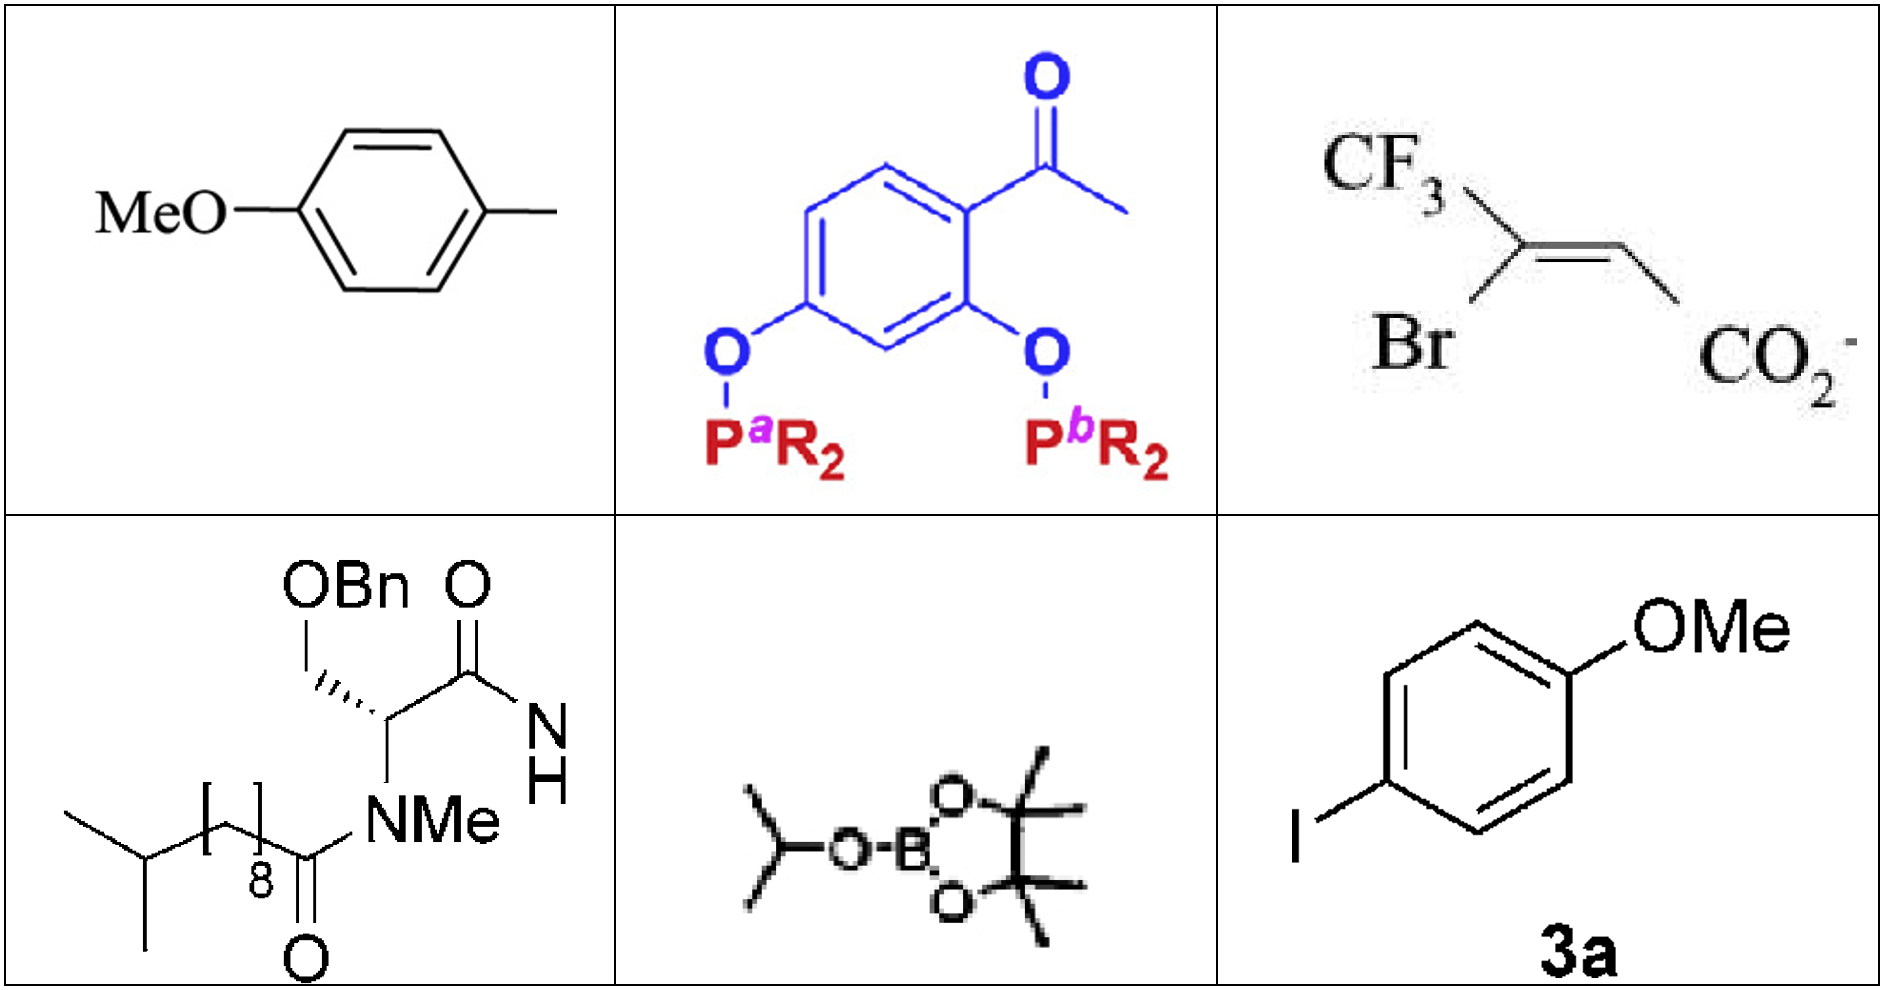
\includegraphics[scale=0.3]{imagenes/positive_examples.png}}  
    \caption{Ejemplos de muestras positivas del dataset} 
\end{figure}

Los ejemplos negativos son, en cambio, imágenes que contienen rectas, curvas y otras figuras que se parecen a las formas que adquiere una molécula, pero no lo son. En esta categoría hay más imágenes, 800 en total.

\begin{figure}[H]
\centering
    \fbox{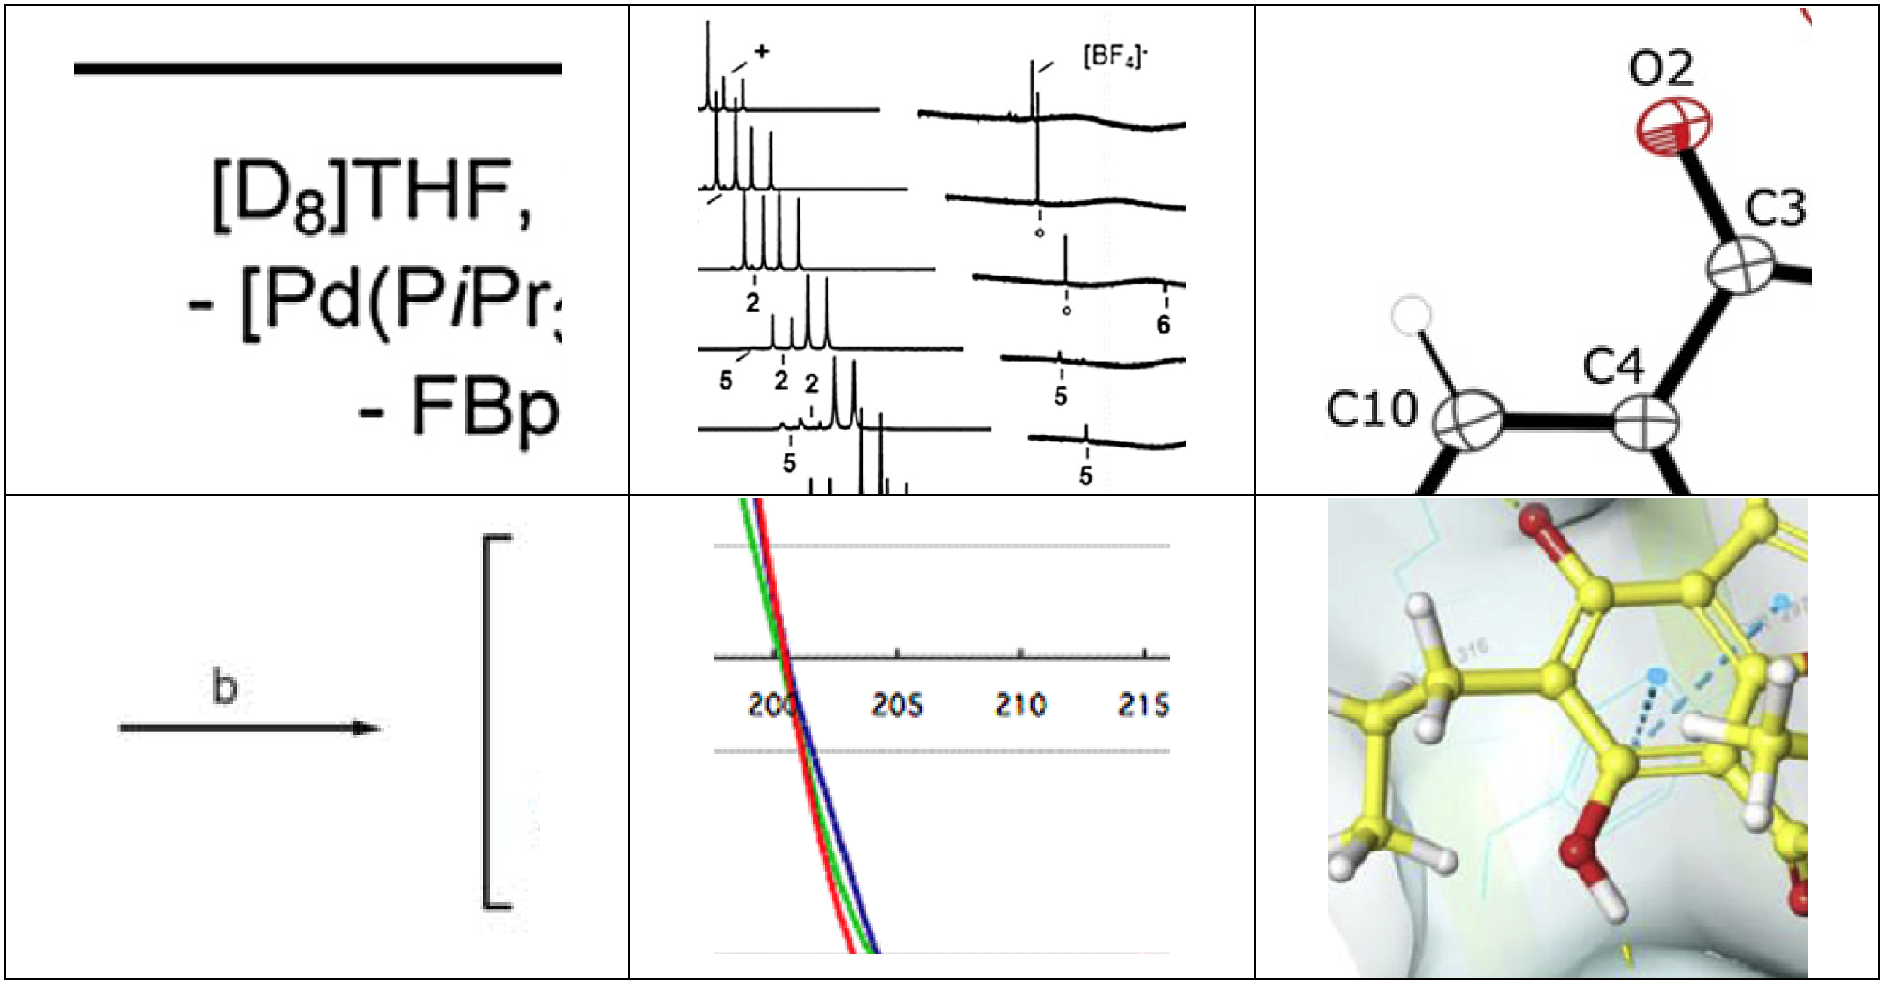
\includegraphics[scale=0.3]{imagenes/negative_examples.png}}  
    \caption{Ejemplos de muestras negativas del dataset} 
\end{figure}

Estas imágenes necesitan un preprocesamiento, es necesario elegir el formato con el que se va a trabajar y dimensionarlas para que todas tengan el mismo tamaño. Debido a que el canal alfa del formato .png no se está aprovechando, decidimos convertirlas a formato .jpg y así trabajar con tres canales en nuestros modelos. Además, el modelo generativo que utilizamos está diseñado para trabajar con imágenes con este número de canales, así que será lo más adecuado.

Lo más conveniente sería dimensionar todas las imágenes al tamaño de la más grande, así no se perdería información. Pero esto puede suponer un problema, ya que existen algunas que superan los 700x700 píxeles, y cuanto mayor es su resolución más parámetros necesitan almacenar los modelos, dando lugar a altos tiempos de ejecución, y sobre todo, a problemas con la memoria de la GPU. Las GPUs del clúster no tienen capacidad para almacenar modelos con tantos parámetros, por lo que decidimos reducir el tamaño de las imágenes a 256x256. 

También mencionar el limitado número de ejemplos positivos que tenemos en comparación con negativos: estamos ante un conjunto de datos desbalanceado. En el momento de entrenar el clasificador, tendremos que conseguir que esté balanceado, ya sea reduciendo el número de ejemplos negativos utilizado o aplicando \textit{data augmentation} sobre los positivos. En este trabajo elegimos la segunda opción, ya que en Aprendizaje Automático cuantos más datos se utilizan en el entrenamiento, mejores modelos se obtienen y con mayor capacidad de generalización. 

La técnica de \textit{data augmentation} consiste en aumentar el tamaño del conjunto de datos completándolo con imágenes alteradas de este. Existen bibliotecas en lenguajes de programación como Python que facilitan en gran medida esta tarea, ya que permiten indicar, entre una serie de transformaciones ya implementadas, cuáles queremos aplicar \cite{imgaug}. En nuestro caso vamos a crear tres \textit{data augmentation} diferentes, y comprobaremos cuál funciona mejor en los experimentos. La primera realizará transformaciones suaves, la segunda algo más fuertes y la tercera bastante disruptivas.

\begin{algorithm}[H]
    \caption{\textit{Data augmentation} 1: Transformaciones suaves}
\begin{algorithmic}[1]
    \State A\_veces(50\%, DesenfoqueGaussiano(sigma=[0, 0.5]))
    \State Escalar(x: [80\%, 100\%], y: [80\%, 100\%])
    \State Rotar([-25º, +25º])
    \State Estirar([-5,5])
\end{algorithmic}
\end{algorithm}

A cada imagen del conjunto de datos se le aplicarán estas cuatro transformaciones, la primera solamente con un 50\% de probabilidad. Los parámetros de cada transformación vienen dados en un rango, de forma que se elige un valor aleatorio en este.

\begin{figure}[H]
\centering
    \begin{subfigure}{.35\textwidth}
        \centering
        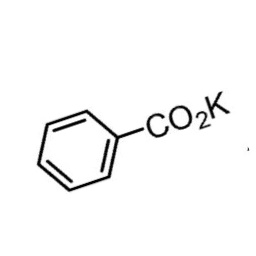
\includegraphics[width=1\linewidth]{imagenes/aug/180.jpg}
    \end{subfigure}%
    \begin{subfigure}{.35\textwidth}
        \centering
        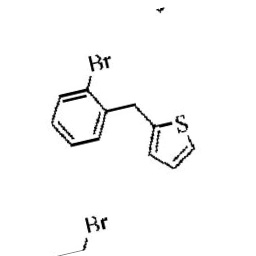
\includegraphics[width=1\linewidth]{imagenes/aug/193.jpg}
    \end{subfigure}%

    \bigskip

    \begin{subfigure}{.35\textwidth}
        \centering
        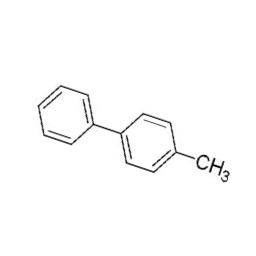
\includegraphics[width=1\linewidth]{imagenes/aug/224.jpg}
    \end{subfigure}%
    \begin{subfigure}{.35\textwidth}
        \centering
        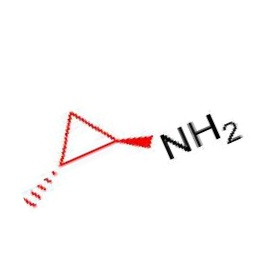
\includegraphics[width=1\linewidth]{imagenes/aug/370.jpg}
    \end{subfigure}

    \caption{Imágenes generadas aplicando \textit{data augmentation} 1}
\end{figure}

Algunos ejemplos son los que se muestran sobre este párrafo, se aprecian leves rotaciones y estiramientos de las imágenes, sin existir gran diferencia con las originales.

\begin{algorithm}[H]
    \caption{\textit{Data augmentation} 2: Transformaciones más fuertes}
\begin{algorithmic}[1]
    \State A\_veces(50\%, DesenfoqueGaussiano(sigma=[0, 0.5]))
    \State ContrasteLineal([0.75, 1.5])
    \State Escalar(x: [70\%, 100\%], y: [70\%, 100\%])
    \State Rotar([-45º, +45º])
    \State Estirar([-10,10])
    \State Trasladar(x: [-10\%, 10\%], y: [-10\%, 10\%])
    \State Multiplicar([0.8, 1.2], por\_canal=25\%)
    \State RuidoGaussianoAditivo(loc=0, escala=[0.0, 0.05*255])
    \State VoltearIzdaDcha(30\%)
\end{algorithmic}
\end{algorithm}

En este caso, utilizaremos transformaciones como Multiplicar (multiplica el valor de los píxeles de la imagen por un número entre 0.8 y 1.2), RuidoGaussianoAditivo (donde a cada píxel se le añade ruido generado mediante una distribución gaussiana centrada en 0 y con desviación entre 0 y 0.05*255) o VoltearIzqdaDcha, entre otras.

\begin{figure}[H]
\centering
    \begin{subfigure}{.35\textwidth}
        \centering
        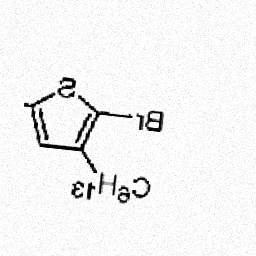
\includegraphics[width=1\linewidth]{imagenes/aug2/169.jpg}
    \end{subfigure}%
    \begin{subfigure}{.35\textwidth}
        \centering
        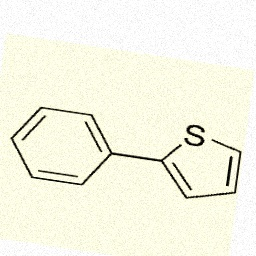
\includegraphics[width=1\linewidth]{imagenes/aug2/188.jpg}
    \end{subfigure}%

    \bigskip

    \begin{subfigure}{.35\textwidth}
        \centering
        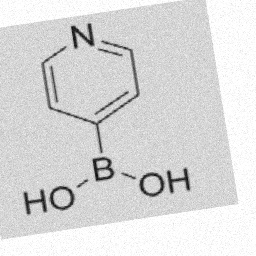
\includegraphics[width=1\linewidth]{imagenes/aug2/221.jpg}
    \end{subfigure}%
    \begin{subfigure}{.35\textwidth}
        \centering
        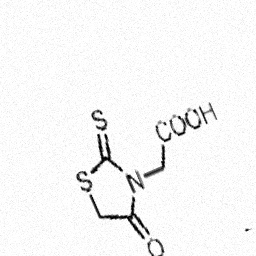
\includegraphics[width=1\linewidth]{imagenes/aug2/222.jpg}
    \end{subfigure}

    \caption{Imágenes generadas aplicando \textit{data augmentation} 2}
\end{figure}

En este caso se observan más cambios fundamentalmente debidos a las variaciones en contraste, al uso de ruido gaussiano y a la multiplicación, responsable de los cambios de color, ya que a veces se aplica a canales independientes. 

\begin{algorithm}[H]
    \caption{\textit{Data augmentation} 3: Transformaciones fuertes}
\begin{algorithmic}[1]
    \State A\_veces(50\%, DesenfoqueGaussiano(sigma=[0, 0.6]))
    \State ContrasteLineal([0.75, 2])
    \State Escalar(x: [70\%, 100\%], y: [70\%, 100\%])
    \State Rotar([-45º, +45º])
    \State Estirar([-10,10])
    \State Trasladar(x: [-20\%, 20\%], y: [-10\%, 10\%])
    \State Multiplicar([0.6, 1.4], por\_canal=25\%)
    \State RuidoGaussianoAditivo(loc=0, escala=[0.0, 0.05*255], por\_canal=30\%)
    \State VoltearIzdaDcha(20\%)
    \State VoldearArribaAbajo(20\%)
    \State A\_veces(70\%, TransformacionElastica(alfa=[0.75, 3], sigma=(0.2, 0.5)))
    \State UnoEntre(Nitidez(alfa=[0, 1], lightness=[0.5, 1.5]), Emboss(alfa=[0, 1], fuerza=[0.75, 2]))
    \State Dropout([0.01, 0.15], por\_canal=0.5)
\end{algorithmic}
\end{algorithm}
% TODO: Cómo se traduce emboss al español??

Finalmente, en esta versión de \textit{data augmentation} añadimos transformaciones que alteran en gran medida el aspecto de las imágenes. TransformacionElastica desplaza píxeles de una zona de la imagen a otra cercana, donde alfa controla la distancia con la que se produce el desplazamiento y sigma la suavidad de este, un valor bajo de sigma dará lugar a imágenes ruidosas y pixeladas. Nitidez aplica este efecto a la imagen y mezcla el resultado con la imagen original, la intensidad de la mezcla se controla con el parámetro alfa, mientras que el parámetro lightness controla el brillo de la imagen. Emboss da a la imagen un aspecto metálico, pronunciando las altas luces y sombras. Por último, Dropout da el valor 0 a cada pixel con una probabilidad entre 0.01 y 0.15. 

\begin{figure}[H]
\centering
    \begin{subfigure}{.35\textwidth}
        \centering
        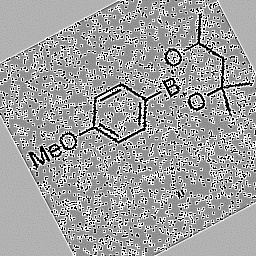
\includegraphics[width=1\linewidth]{imagenes/aug3/175.jpg}
    \end{subfigure}%
    \begin{subfigure}{.35\textwidth}
        \centering
        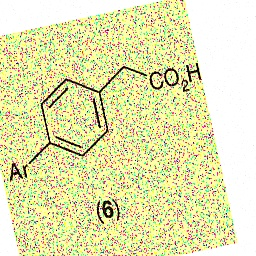
\includegraphics[width=1\linewidth]{imagenes/aug3/183.jpg}
    \end{subfigure}%

    \bigskip

    \begin{subfigure}{.35\textwidth}
        \centering
        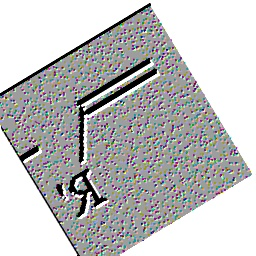
\includegraphics[width=1\linewidth]{imagenes/aug3/225.jpg}
    \end{subfigure}%
    \begin{subfigure}{.35\textwidth}
        \centering
        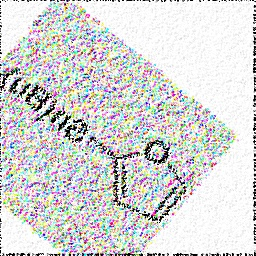
\includegraphics[width=1\linewidth]{imagenes/aug3/271.jpg}
    \end{subfigure}

    \caption{Imágenes generadas aplicando \textit{data augmentation} 3}
\end{figure}

En esta última versión las transformaciones son bastante agresivas. Se introduce mucho ruido en las imágenes y las rotaciones y los cambios en el contraste son fuertes.

\section{Estructura del código}
Como se menciona al principio del capítulo, la implementación se sitúa en el directorio $experiments/$, dividido en dos subdirectorios. El primero contiene el código del modelo generador de imágenes, el segundo el del clasificador: \\

\dirtree{%
    .1 experiments/\DTcomment{implementación del TFG}.
    .2 taming\_transformers/\DTcomment{generador de imágenes}.
    .3 taming-transformers/.
    .4 configs/.
    .4 logs/.
    .4 train\_ngpu.sh.
    .3 data\_generation\_and\_aug.ipynb.
    .3 sample\_and\_clean\_molecules.ipynb.
    .3 sampling\_experiment.ipynb.
    .3 functions.py.
    .2 image\_classifier/\DTcomment{clasificador de imágenes}.
    .3 saved\_models/.
    .3 datasets.py.
    .3 functions.py.
    .3 grid\_search.py.
    .3 models.py.
    .3 train.py.
    .3 train\_ngpu.sh.
}

\subsection{Generador de imágenes sintéticas}
Uno de los objetivos del proyecto es construir un modelo que nos permita generar imágenes sintéticas de moléculas. 

\section{Ejecución y reproducibilidad}
Como ejecutar los scripts y semillas utilizadas